\chapter{Evaluation}\label{chapter:Evaluation}
For the evaluation of the algorithms some parameters should be chosen in order to get reasonable results. The edge-weight distribution is always set to be a uniform distribution on $[0.1, 1.1]$. As long as not mentioned differently, $n = 20, r = 3, d = 3, k = 3$.  The choices of the constants are justified in the respecting sections.



\section{Input graph sizes}
For evaluating the implementation of \cref{alg:ses} in comparison to the brute-force solution, the maximal size of graphs (in $n$) which can be brute-forced in a reasonable time is determined. In general, it is favourable to generate as large as possible graphs in order to see how the algorithm performs.

However, the as the brute forcing time correlates with around $ \mathcal{O}(2^n)$, with the available resources, for $n=20$ brute-forcing already took around 18 s compared to 38 s for computing a small set expansion. As the brute-forcing time roughly doubles for each additional vertex, it is unfeasible to set $n$ much higher. Even though 21 vertices would be possible, due to \cref{eq:ndmr} an uneven number would unnecessarily limit the possible combinations of ranks and degree as evaluated in \cref{fig:rank_degree_times}, as for example, there would be no integer value for m if n = 21, d= 3 and r = 6.

Aditionally for analyzing the constant in \cref{fact:small_xi}, a plot of as many graps as possible seems to be ideal. So not only for brute-forcing but also for executing the estimation algorithm, the graph shouldn't be too big. In conclusion, half a minute seems to be a reasonable time for one run of the algorithm. % as the time complexity of the small set expansion approcximation implementation shows to be at around ... $n...$
The times needed for different number of vertices can be seen in \cref{fig:no_vertices_time}.
\begin{figure}[htpb]
	\centering
	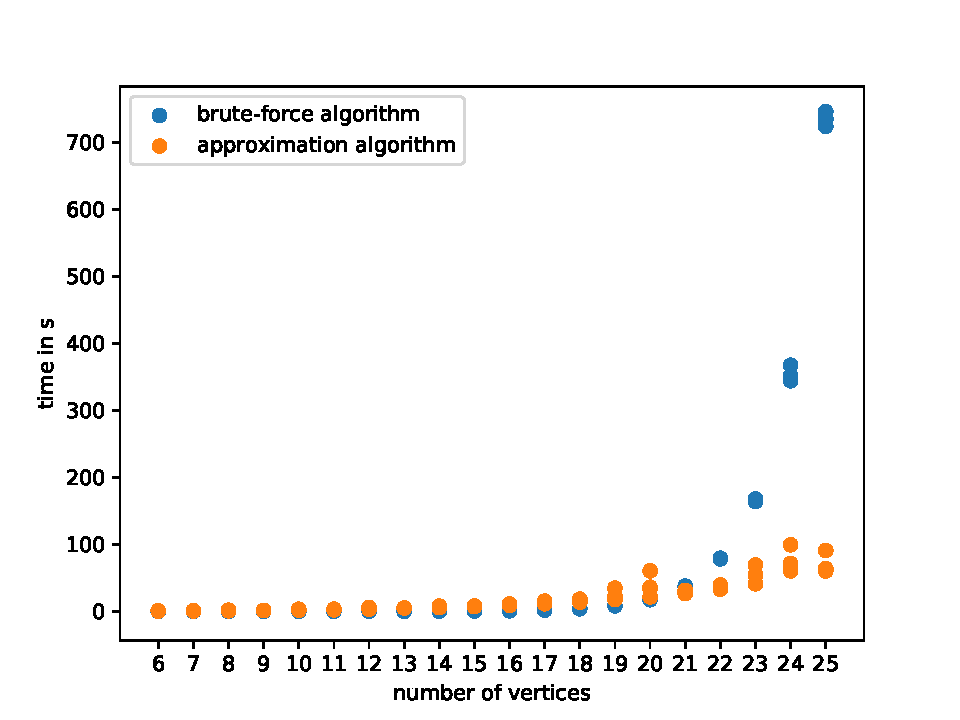
\includegraphics[scale=0.8]{figures/number_vertices_all_logs.pdf}
	\caption[Plot graph size vs time]{Plot of the number of vertices $n$ against the time for computing solutions. It can be seen that the brute-force algorithm takes a long time for larger graphs, while the approximation algorithm's time only increases slowly.\label{fig:no_vertices_time}}
\end{figure}

Therefore $n$ is set to be 20 for further analysis.
\section{Rank degree combinations}

As the graphs generated by the algorithms have uniform ranks and regular degrees, it needs to be determined which combination of r and d should be chosen. As already mentioned, they can not be chosen freely, not for all combinations r-uniform d-regular graphs exist on n vertices, e of equation \cref{eq:ndmr}. 
As all of the variables need to be non-negative integers, one can ensure to never violate that constraint for any $n$ by setting $d=r$. An evaluation of the time constraints can be seen in \cref{fig:rank_degree_times}. Interestingly, for equal r and d, the brute-force algorithm's time did almost not increase when d and r were increased from (2,2) to (8,8). The small set approximation algorithm's times however, seem to increase linearly with r and d. For other combinations, the brute-force algorithm needed more time for comparatively high $\frac{d	}{r}$ ratios.

For easier evaluation of the other properties, the rank and degree were chosen to be $r=3$ and $d=3$, as with a rank of 3 it is explicitly demonstrated that the algorithms work on hypergraphs.
\begin{figure}
	\centering
	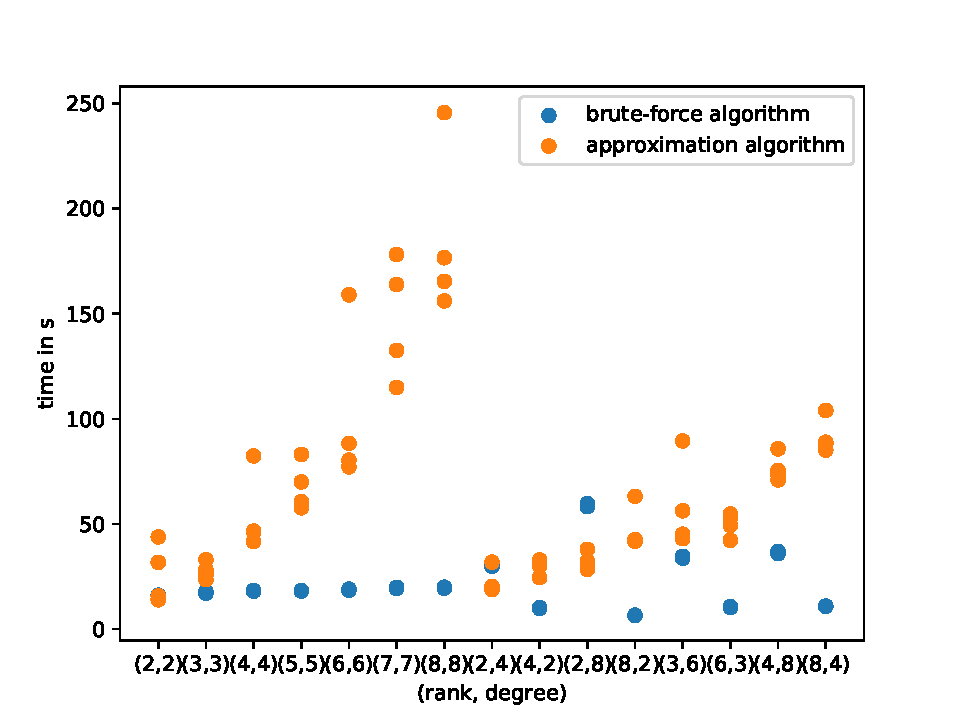
\includegraphics[scale=0.8]{figures/rank_degree_combinations_all_logs.pdf}
	\caption[Plot times rank degree combinations]{Plot of times for rank degree combinations.\label{fig:rank_degree_times}}
\end{figure}


\section{Evaluation of k}

The value of k plays an important role in the properties of the graph as well as the runtime. As described in \cref{alg:procedural_minimizer}, k vectors are constructed.
As for k = 1, no SDP must be solved, the algorithm terminates quickly. However, this does not make sense anyways, as \cref{fact:small_xi} does only hold for $k\ge2$.
As seen in \cref{fig:k_time}, for higher k, the time for each small expansion set approximation increases. Profiling the algorithm also showed that most of the time was spent on solving the SDP. Unfortunately for higher k, the optimization takes unreasonably long, presumably due to numerical instabilities.

\begin{figure}
	\centering
	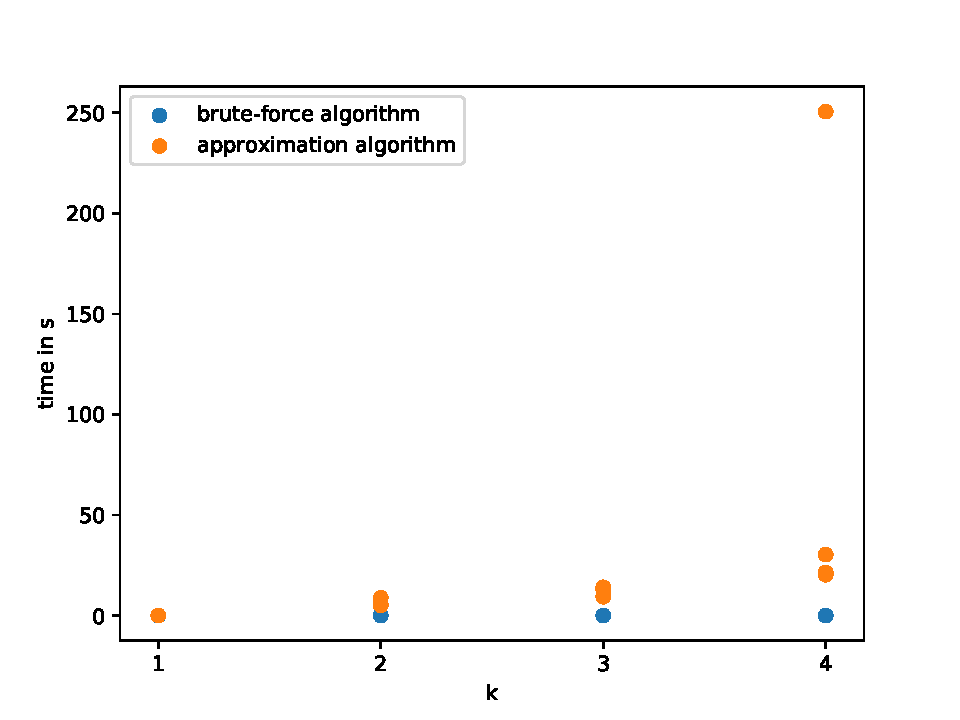
\includegraphics[scale=0.8]{figures/k_all_logs.pdf}
	\caption[Plot k time ]{Plot of k against time.\label{fig:k_time}}
\end{figure}

\section{Small expansion sizes}

As seen in \cref{fig:sizes_small_expansions}, most of the sampled small expansion sets have a small number of vertices. TODO: verify: As k increases, this trend continues, going along the trend of getting smaller sets for larger k as indicated in \cref{fact:small_xi}.


Since higher values of k were not feasible in \cref{eq:small_expansion} due to numerical issues of the implementation as well as time constraints, $|S|<\frac{24|V|}{k}$ can't be verified as k<5 here.
C is desirable, as it would lead to small expansions.

\begin{figure}
	\centering
	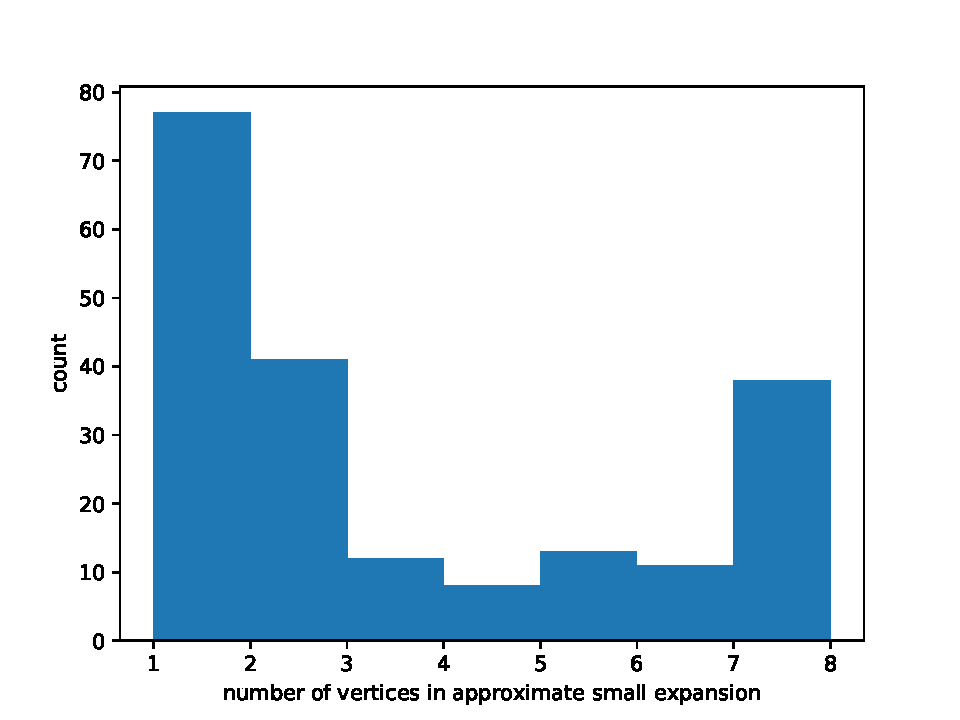
\includegraphics[scale=1]{figures/quality_evaluation_log_small_expansion_sizes.pdf}
	\caption[Plot sizes small expansions]{Plot of sizes of small expansions.\label{fig:sizes_small_expansions}}
\end{figure}


\section{Random graphs comparison}
As the expansion for non-connected graphs is always 0, only algorithms which guarantee to return connected graphs will be considered, namely \ref{alg:GenerateRandomGraphWithResampling}, \ref{alg:swap_edges} and \ref{alg:spanning_tree}.

The expansion of the graphs is be evaluated against each other via brute-force. The results can be seen in \cref{fig:plot_lowest_expansion_each_size}.

\begin{figure}
	\centering
	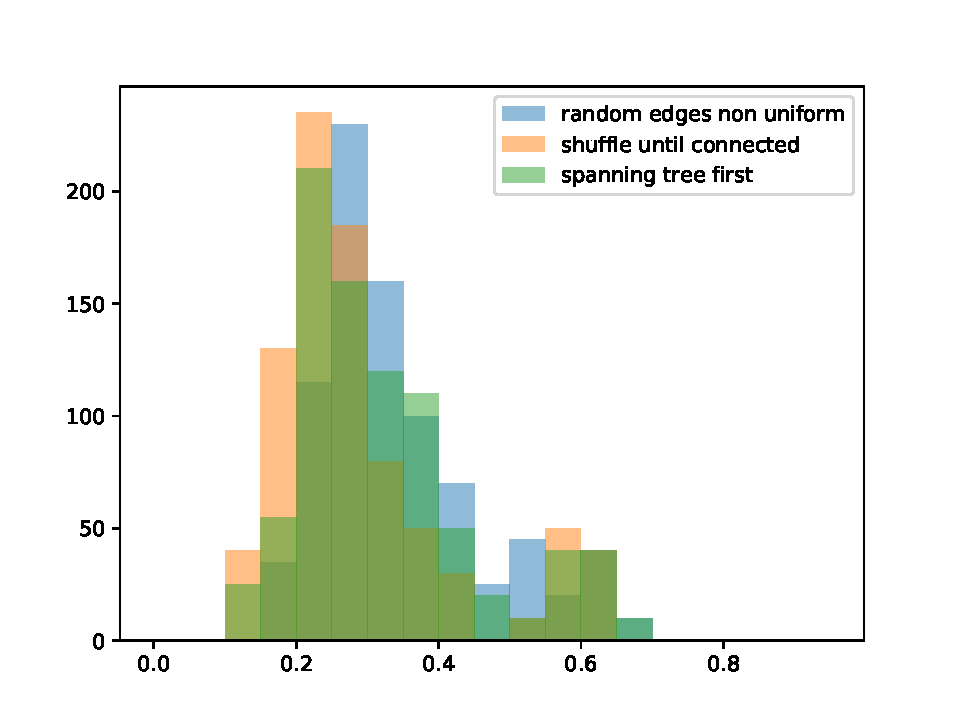
\includegraphics[scale=1]{figures/creation_algorithm_log_lowest_expansion.pdf}
	\caption[Plot lowest expansion for different algorithms]{Plot of the lowest expansion values of the graphs created by different algorithms for each size of the expansion set. \cref{fig:plot_lowest_expansion_each_size}}
\end{figure}

\section{Estimation of C}
As according to \cref{fact:small_xi} a small value of C would be favourable to ensure small estimated expansions. 
For estimating $C$, the inequality of \cref{fact:small_xi} can be changed to:
\begin{equation} \label{eq:c_estimate}
C\ge \frac {\phi(S)}{ \min\{\sqrt{r \log k}, k \log k  \log \log k \sqrt{\log r} \} \cdot \sqrt{\xi}}
\end{equation} $\log$ refers to the natural logarithm here.


However, \cref{fig:c_estimates} does not show a clear picture. Since all the results were between ... and ..., one could hypothesize that C is at max .... TODO


\begin{figure}
	\centering
	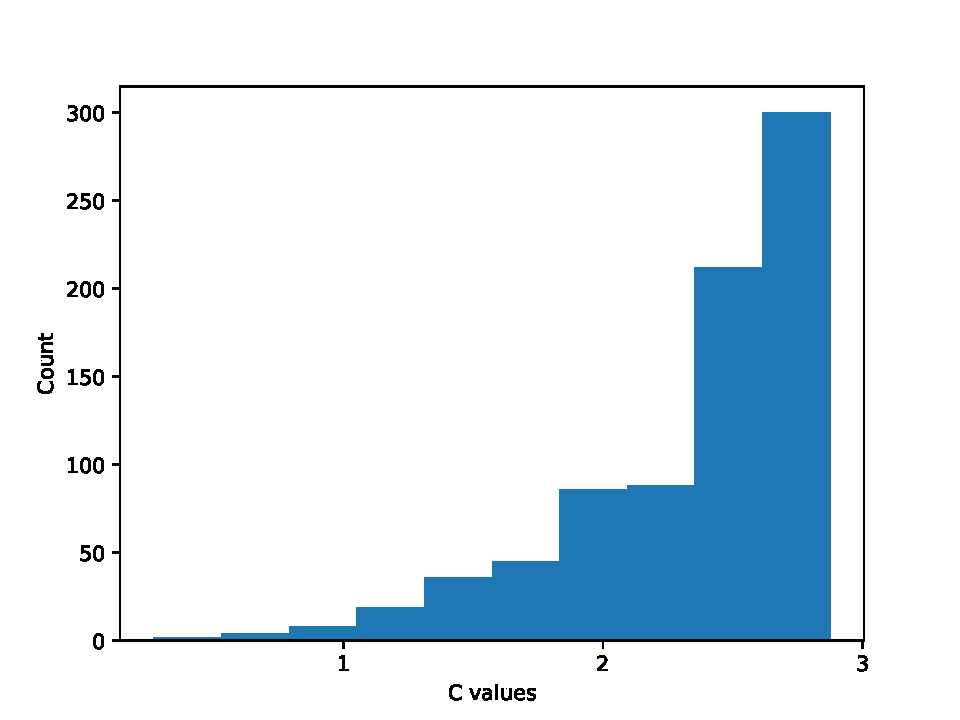
\includegraphics[scale=1]{figures/quality_evaluation_log_C_estimates.pdf}
	\caption[Plot C estimates]{Plot of estimates for C\label{fig:c_estimates}}
\end{figure}





\section{Comparison of expansion values}




Finally, the quality of the results is analyzed. As seen in \cref{fig:expansion_approx_vs_brute}, the set with the lowest expansion value found by the brute force algorithm is, as expected, always at least as low as the value found by the approximation algorithm. Howeverm when comparing the best expansion values against the best one-percentile value as found by the brute-force algorithm, the approximation algorithm performs better ...\% of times. However, the approximation algorithm



TODO

Therefore improvements

\begin{figure}
	\centering
	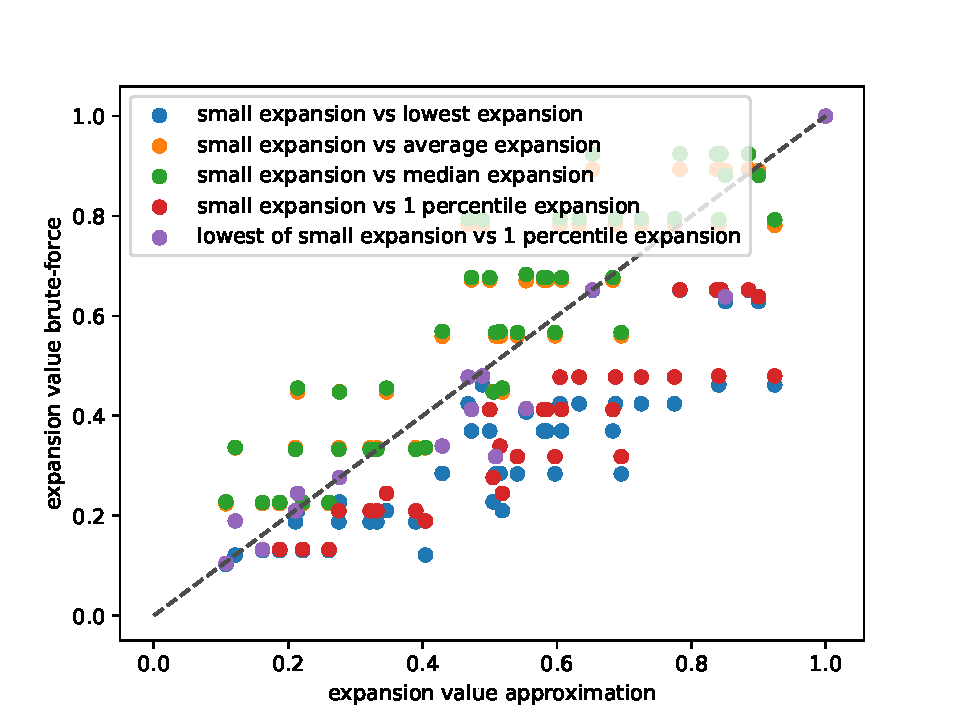
\includegraphics[scale=1]{figures/quality_evaluation_log_expansion_values_for_same_number_verticies.pdf}
	\caption[Plot expansions approximation vs brute force]{Plot of the expansion values achieved by the small expansion set approximation algorithm against the expansion set of the same size with the lowest expansion (as generated through the brute-force approach).  Entries below the line signal that the expansion found by the approximation algorithm was worse than the set found by the brute force algorithm. \label{fig:expansion_approx_vs_brute}}
\end{figure}




